\section{Computational Aerodynamic Pipeline and Multi-Fidelity Hierarchy}
\label{sec:pipeline}

\subsection{3D Vortex Lattice Formulation and Mesh Discretization}
\label{sec:vlm_discretization}
Aerodynamic lifting forces and induced drag are calculated using the 3D Vortex Lattice Method (VLM) implemented within the AeroSandbox computational framework~\cite{sharpe2021aerosandbox}. The VLM represents the vehicle lifting surface by a distribution of horseshoe vortex filaments arranged on planar panels along the mean camber surface, enforcing the Neumann boundary condition of zero normal velocity (flow tangency) at panel collocation points~\cite{katz2001low}:
\begin{equation}
(\mathbf{V}_\infty + \mathbf{v}_{\mathrm{induced}}) \cdot \mathbf{n}_i = 0
\end{equation}
where $\mathbf{n}_i$ is the unit normal vector of panel $i$, $\mathbf{V}_\infty$ is the freestream velocity, and $\mathbf{v}_{\mathrm{induced}}$ is the total velocity induced by all horseshoe vortex filaments governed by the Biot--Savart law.

\begin{figure}[htbp]
\centering
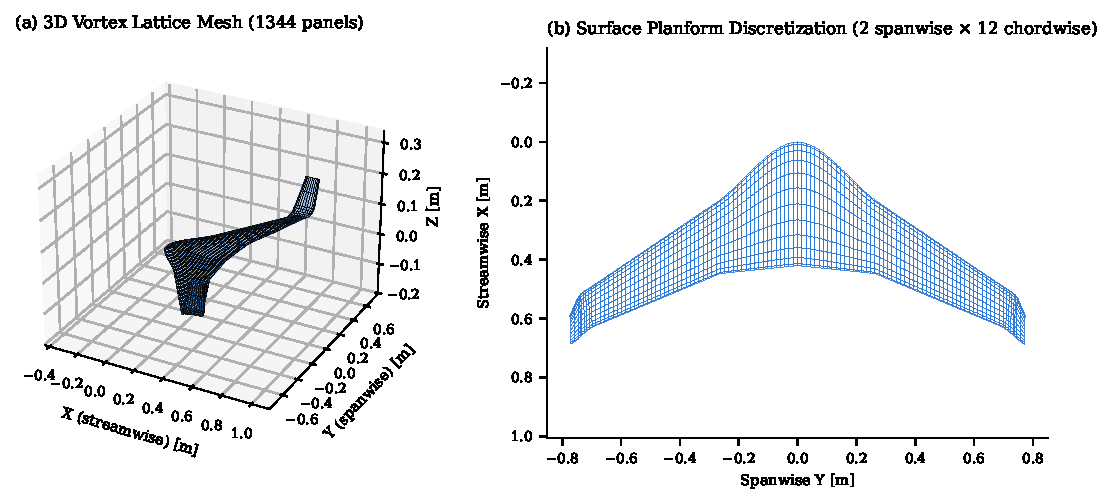
\includegraphics[width=\linewidth]{figures/fig_vlm_discretization.pdf}
\caption{Computational surface panel discretization of the tailless BWB UAV. (a) 3D isometric perspective showing chordwise and spanwise panel distributions across the center-body, outer wing, and canted winglet surfaces. (b) 2D planform projection illustrating cosine panel clustering along the leading and trailing edges ($N_{\mathrm{panels}} = 1{,}344$).}
\label{fig:vlm_discretization}
\end{figure}

As illustrated in Fig.~\ref{fig:vlm_discretization}, the wing is defined by 29 sections per side (25 equally spaced stations on the main wing, three on the circular-arc winglet junction and one at the winglet tip), which gives 28 section intervals. The production discretization uses 2 spanwise panels per interval and 12 chordwise panels, that is 672 panels per side and $1{,}344$ in total ($1{,}152$ on the main wing and $192$ on the winglet junction and winglets).
Chordwise panel distribution employs cosine spacing, clustering panels densely at the leading edge to capture suction peaks and at the trailing edge to enforce the Kutta condition accurately. Spanwise panel boundaries are aligned with structural section breaks to prevent geometric skewness. The sensitivity of aerodynamic coefficients and static margin to panel resolution is formally quantified in the 7-level grid convergence audit of Section~\ref{sec:grid_convergence}.

\subsection{Longitudinal Stability and Trim Derivation}
For unaccelerated level flight at cruise speed $V$, the vehicle must generate the required equilibrium lift coefficient:
\begin{equation}
C_{L,\mathrm{cruise}} = \frac{2 m g}{\rho V^2 S_{\mathrm{ref}}}
\end{equation}
Because the lattice lift is linear in the angle of attack, the pipeline evaluates $C_L$ at $\alpha = 0^\circ$ and $5^\circ$ and interpolates linearly to the angle $\alpha_{\mathrm{cruise}}$ at which $C_L(\alpha_{\mathrm{cruise}}) = C_{L,\mathrm{cruise}}$; a design is rejected if this angle falls outside $[-15^\circ, 20^\circ]$. A third lattice solution at $\alpha_{\mathrm{cruise}}$ gives the forces, the pitching moment about the center of gravity and the stability derivatives.

The longitudinal aerodynamic neutral point $x_{\mathrm{np}}$ follows from the finite-difference stability derivatives that AeroSandbox computes about the cruise point:
\begin{equation}
x_{\mathrm{np}} = x_{\mathrm{ref}} - \bar{c} \cdot \frac{\partial C_m / \partial \alpha}{\partial C_L / \partial \alpha}
\end{equation}
where $x_{\mathrm{ref}}$ is the moment reference point, here the center of gravity $x_{\mathrm{cg}}$, $\bar{c}$ is the mean aerodynamic chord, and $\partial C_m / \partial \alpha$ and $\partial C_L / \partial \alpha$ are the stability derivatives about that point. The longitudinal static margin is then defined non-dimensionally as:
\begin{equation}
SM = \frac{x_{\mathrm{np}} - x_{\mathrm{cg}}}{\bar{c}}
\end{equation}
Constraint Eq.~\eqref{eq:con_sm} enforces $SM \in [0.05, 0.25]$, guaranteeing static pitch stability while preventing excessive pitch stiffness that would degrade maneuvering authority or impose severe trim drag.

\subsection{Viscous Profile Drag and Strip Theory Integration}
Inviscid vortex lattice methods capture induced vortex drag $C_{D,\mathrm{ind}}$ but omit viscous shear stresses and pressure drag arising from boundary-layer development. To capture total cruise drag, the pipeline couples the VLM induced drag with a 2D strip-theory viscous drag integration:
\begin{equation}
C_{D,\mathrm{total}} = C_{D,\mathrm{ind}} + C_{D0} + C_{D,\mathrm{trim}}
\end{equation}
The parasite drag $C_{D0}$ is evaluated by integrating local section profile drag across spanwise strips:
\begin{equation}
C_{D0} = \frac{2}{S_{\mathrm{ref}}} \int_0^{b/2} c(y) \cdot c_{d,\mathrm{profile}}(y) \, dy
\end{equation}
where the local section drag follows a flat-plate skin-friction estimate with a form factor~\cite{raymer2018aircraft}. With the strip Reynolds number $Re_c = V c / \nu$ and the section thickness ratio $\tau$,
\begin{equation}
C_f = x_{\mathrm{tr}}\,\frac{1.328}{\sqrt{x_{\mathrm{tr}} Re_c}} + (1 - x_{\mathrm{tr}})\,\frac{0.455}{(\log_{10} Re_c)^{2.58}}, \qquad c_{d,\mathrm{profile}} = 2\,(1 + 0.2\,\tau)\,\big(1 + 2\tau + 60\tau^4\big)\, C_f
\end{equation}
with an assumed transition location $x_{\mathrm{tr}} = 0.40$ on every strip; the factor $2(1 + 0.2\tau)$ is the wetted-area ratio and the last bracket the form factor. No compressibility correction is applied ($M \approx 0.11$). The skin friction and form drag of the motor boom, motor body and spinner fairing are added in the same way. Trim drag is estimated from the residual cruise pitching moment as $C_{D,\mathrm{trim}} = C_m^2 / (\pi A\!R\, e_{\delta}\, f_{\delta})$ with an elevon effectiveness $e_{\delta} = 0.60$ and an elevon area fraction $f_{\delta} = 0.20$; no control surface is deflected in the lattice model.

\subsection{Independent Models Used for Verification}
\label{sec:mf_tools}
Three tools check the low-order pipeline, and none of them is used inside the optimization: AeroBuildup, the viscous strip method of AeroSandbox; NeuralFoil section polars with predicted transition~\cite{sharpe2024neuralfoil}; and inviscid Euler solutions with SU2~\cite{economon2016su2} on unstructured meshes of about $1.2 \times 10^5$ nodes generated with Gmsh~\cite{geuzaine2009gmsh}. Supplementary Section~\ref{sec:mf_architecture} gives the solver settings. Section~\ref{sec:validation} and Supplementary Sections~\ref{sec:grid_convergence} to~\ref{sec:cfd_validation} use these tools to check the ranking and the constraint values produced by the pipeline.
